%\begin{figure}[!htpb]
%\includegraphics[width=0.7\textwidth]{figures/ATLAS_DarkMatter_Summary_Vector.pdf}\\
%\includegraphics[width=0.7\textwidth]{figures/ATLAS_DarkMatter_Summary_Vector_ModifiedCoupling.pdf}
%\caption{
Regions in DM mass--\Zprime mediator mass
excluded at 95\% CL by a selection of ATLAS searches 
(from References \cite{ATLAS:2016bvn,Aaboud:2018fzt,Aaboud:2017yvp,
Aaboud:2017phn,ATLAS-CONF-2018-005,Aaboud:2017bja,Aaboud:2017dor,
Aaboud:2017buh}) 
available as of July 2018, for two coupling scenarios. Dashed curves labeled ``thermal
relic'' indicate combinations of DM and mediator mass
that are consistent with a DM density of $\omega_c = 0.12
h^2$ and a standard thermal history, as computed in MadDM for this
model~\cite{Backovic:2015cra}. The dotted curve indicates the
kinematic threshold where the mediator can decay on-shell into
DM. 
In panel (a), the couplings of the mediator particle to each generation
of quarks (\gq) are set to 0.25, the couplings to leptons (\gl)
are set to zero and the coupling to DM is set to unity. 
In panel (b), \gq is set to 0.1, \gl is set to 0.01
and the coupling to DM \gdm is set to unity and marked as $g_{DM}$ in this plot.
Abbreviations:\ DM, dark matter; ISR, initial-state radiation; 
TLA, trigger-object level analysis. Adapted from~Reference \citen{ATLASSummary}.
%}
%\label{fig:sensitivityComparison}
%\end{figure}